\section{Durchführung}
\label{sec:Durchführung}

\subsection{Fourier-Synthese}
Für diesen Teil des Experiments werden das Oszilloskop, der Oberwellengenerator
(siehe \autoref{fig:1}) sowie das Multimeter genutzt. Zu Untersuchen sind die
Rechteck-, Sägezahn- und Dreieckspannung.
Der Oberwellengenerator wird als erstes mit dem 
Multimeter verbunden, woraufhin an diesem die höchstmögliche Spannungsamplitude 
eingestellt wird. Bei Kanal eins befindet sich nun die Spannungsamplitude zu
dem Fourierkoeffizienten $a_1$. Im Folgenden wird dann für die jeweiligen Kanäle 
bei der Rechteck-und Sägezahnspannung mit der Ordnung $n$ das $\frac{1}{n}$-fache
dieser Amplitude eingestellt. Bei der Dreieckspannung werden für die Kanäle 
allerdings das $\frac{1}{n^2}$-fache eingestellt. Detektiert werden die Amplituden 
mithilfe des Multimeters.
\begin{figure}
    \caption{Der Oberwellengenerator.}
    \centering
    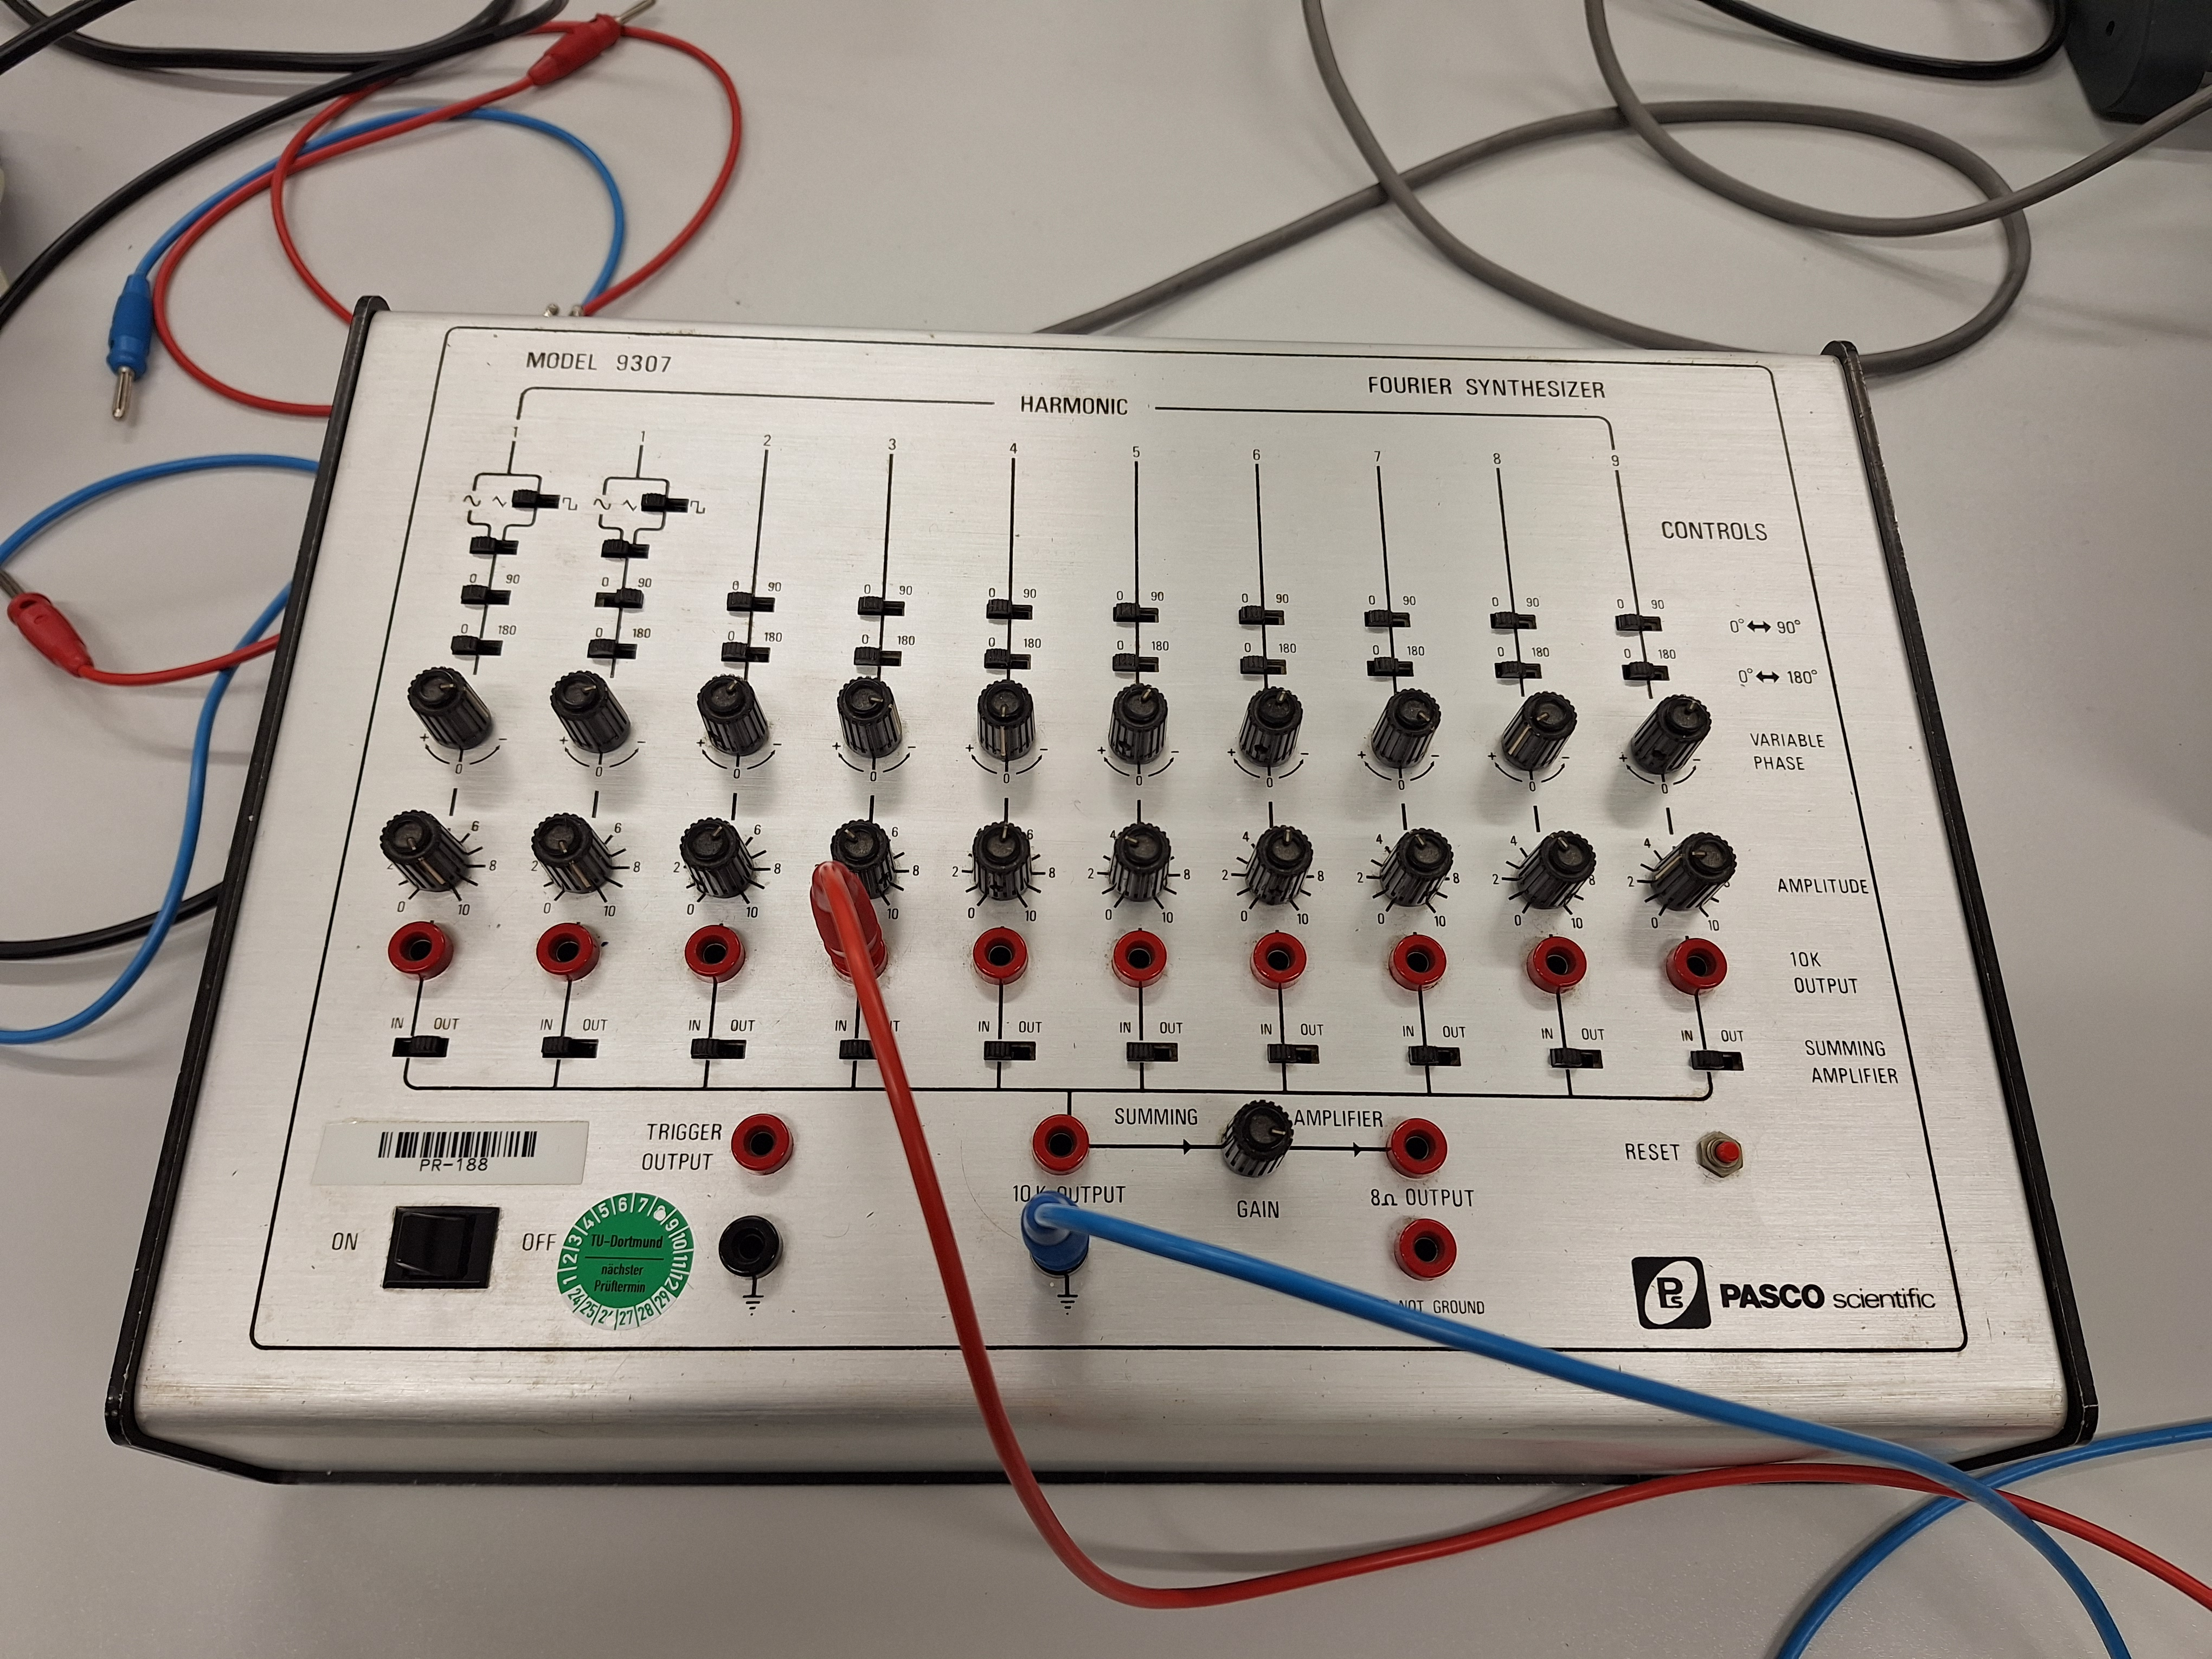
\includegraphics[width=0.7\textwidth]{"Bilder/owg.jpg"}
    \label{fig:1}
\end{figure}
Darauffolgend wird der Oberwellengenerator vom Multimeter getrennt und 
stattdessen mit dem Oszilloskop verbunden. Die Phasenverhältnisse der 
Grundschwingung auf Kanal eins werden mit den restlichen Kurven eingestellt, 
indem auf den X-Eingang des Oszilloskops die Oberwelle des ersten Kanals gesetzt 
wird. Die $n$-te Oberwelle des $n$-ten Kanals befindet sich auf dem Y-Eingang.
Auf dem Oszilloskop sind nun die Lissajous-Figuren zu sehen (eine beliebige ist 
in \autoref{fig:2} zu sehen). Grundsätzlich entstehen sie durch die Überlagerung 
zweier orthogonaler harmonischer Schwingungen.
% \begin{figure}[H]
%     \caption{Lissajous-Figur \cite{lissajous}.}
%     \centering
%     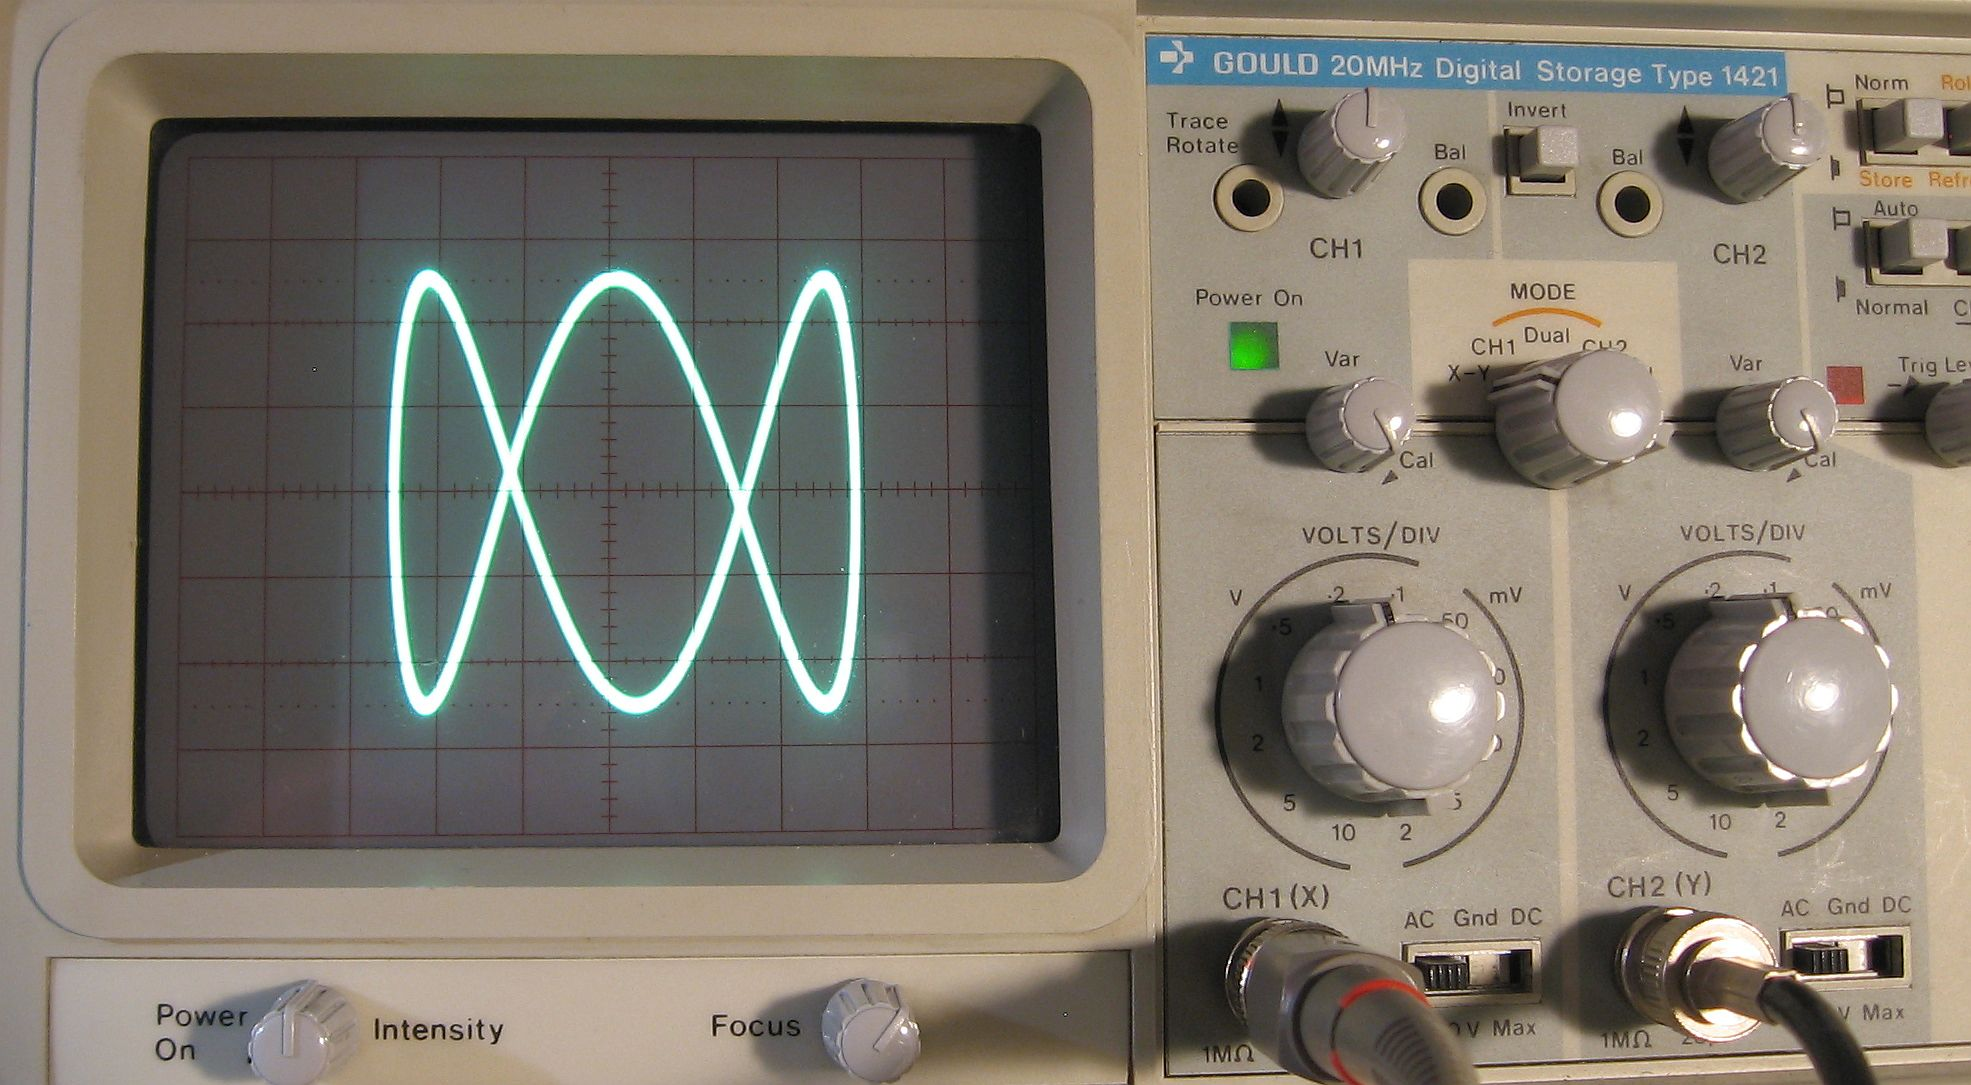
\includegraphics[width=\textwidth]{"Bilder/lissajous.jpg"}
%     \label{fig:2}
% \end{figure}
\begin{figure}[H]
    \centering
    % Erstes Bild
    \begin{minipage}{0.48\textwidth}
        \centering
        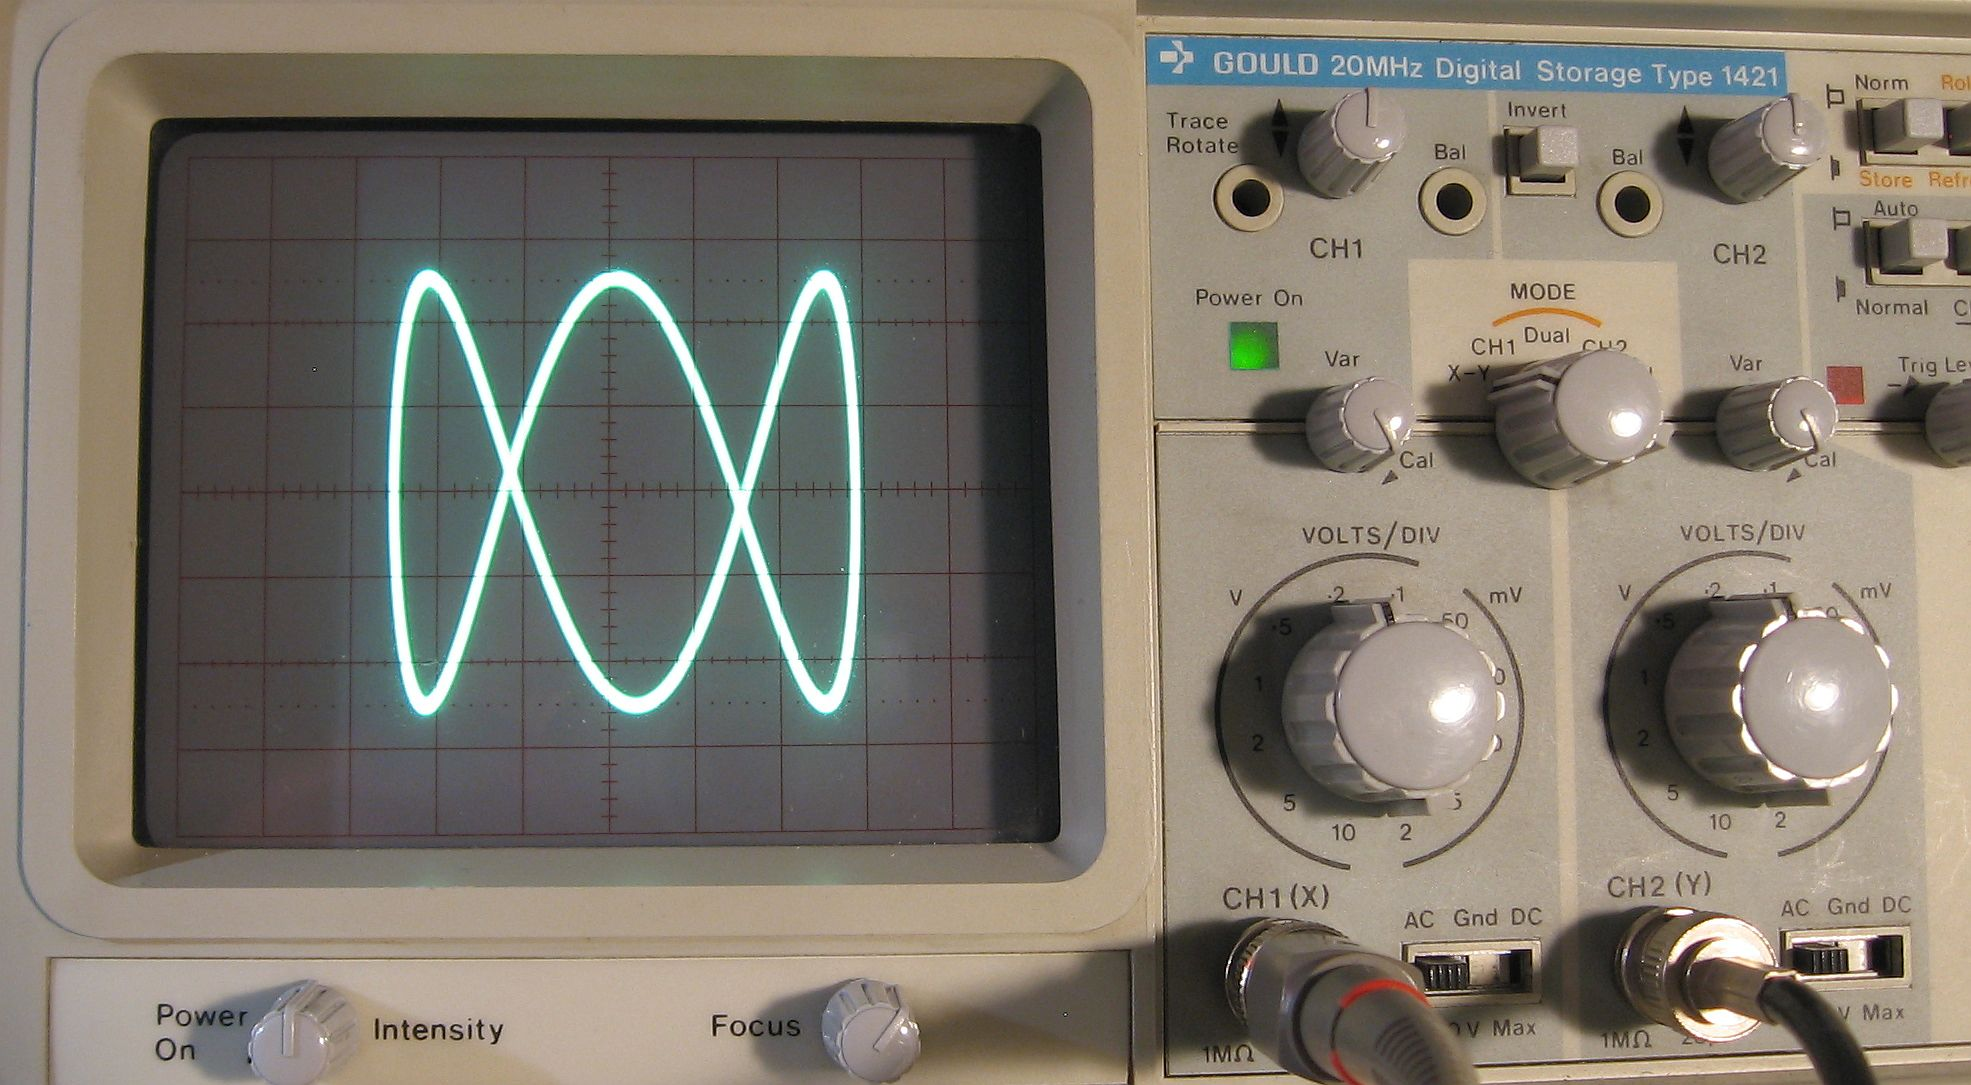
\includegraphics[width=\linewidth]{"Bilder/lissajous.jpg"}
        \caption{Lissajous-Figur \cite{lissajous}.}
        \label{fig:2}
    \end{minipage}
    \hfill
    % Zweites Bild
    \begin{minipage}{0.48\textwidth}
        \centering
        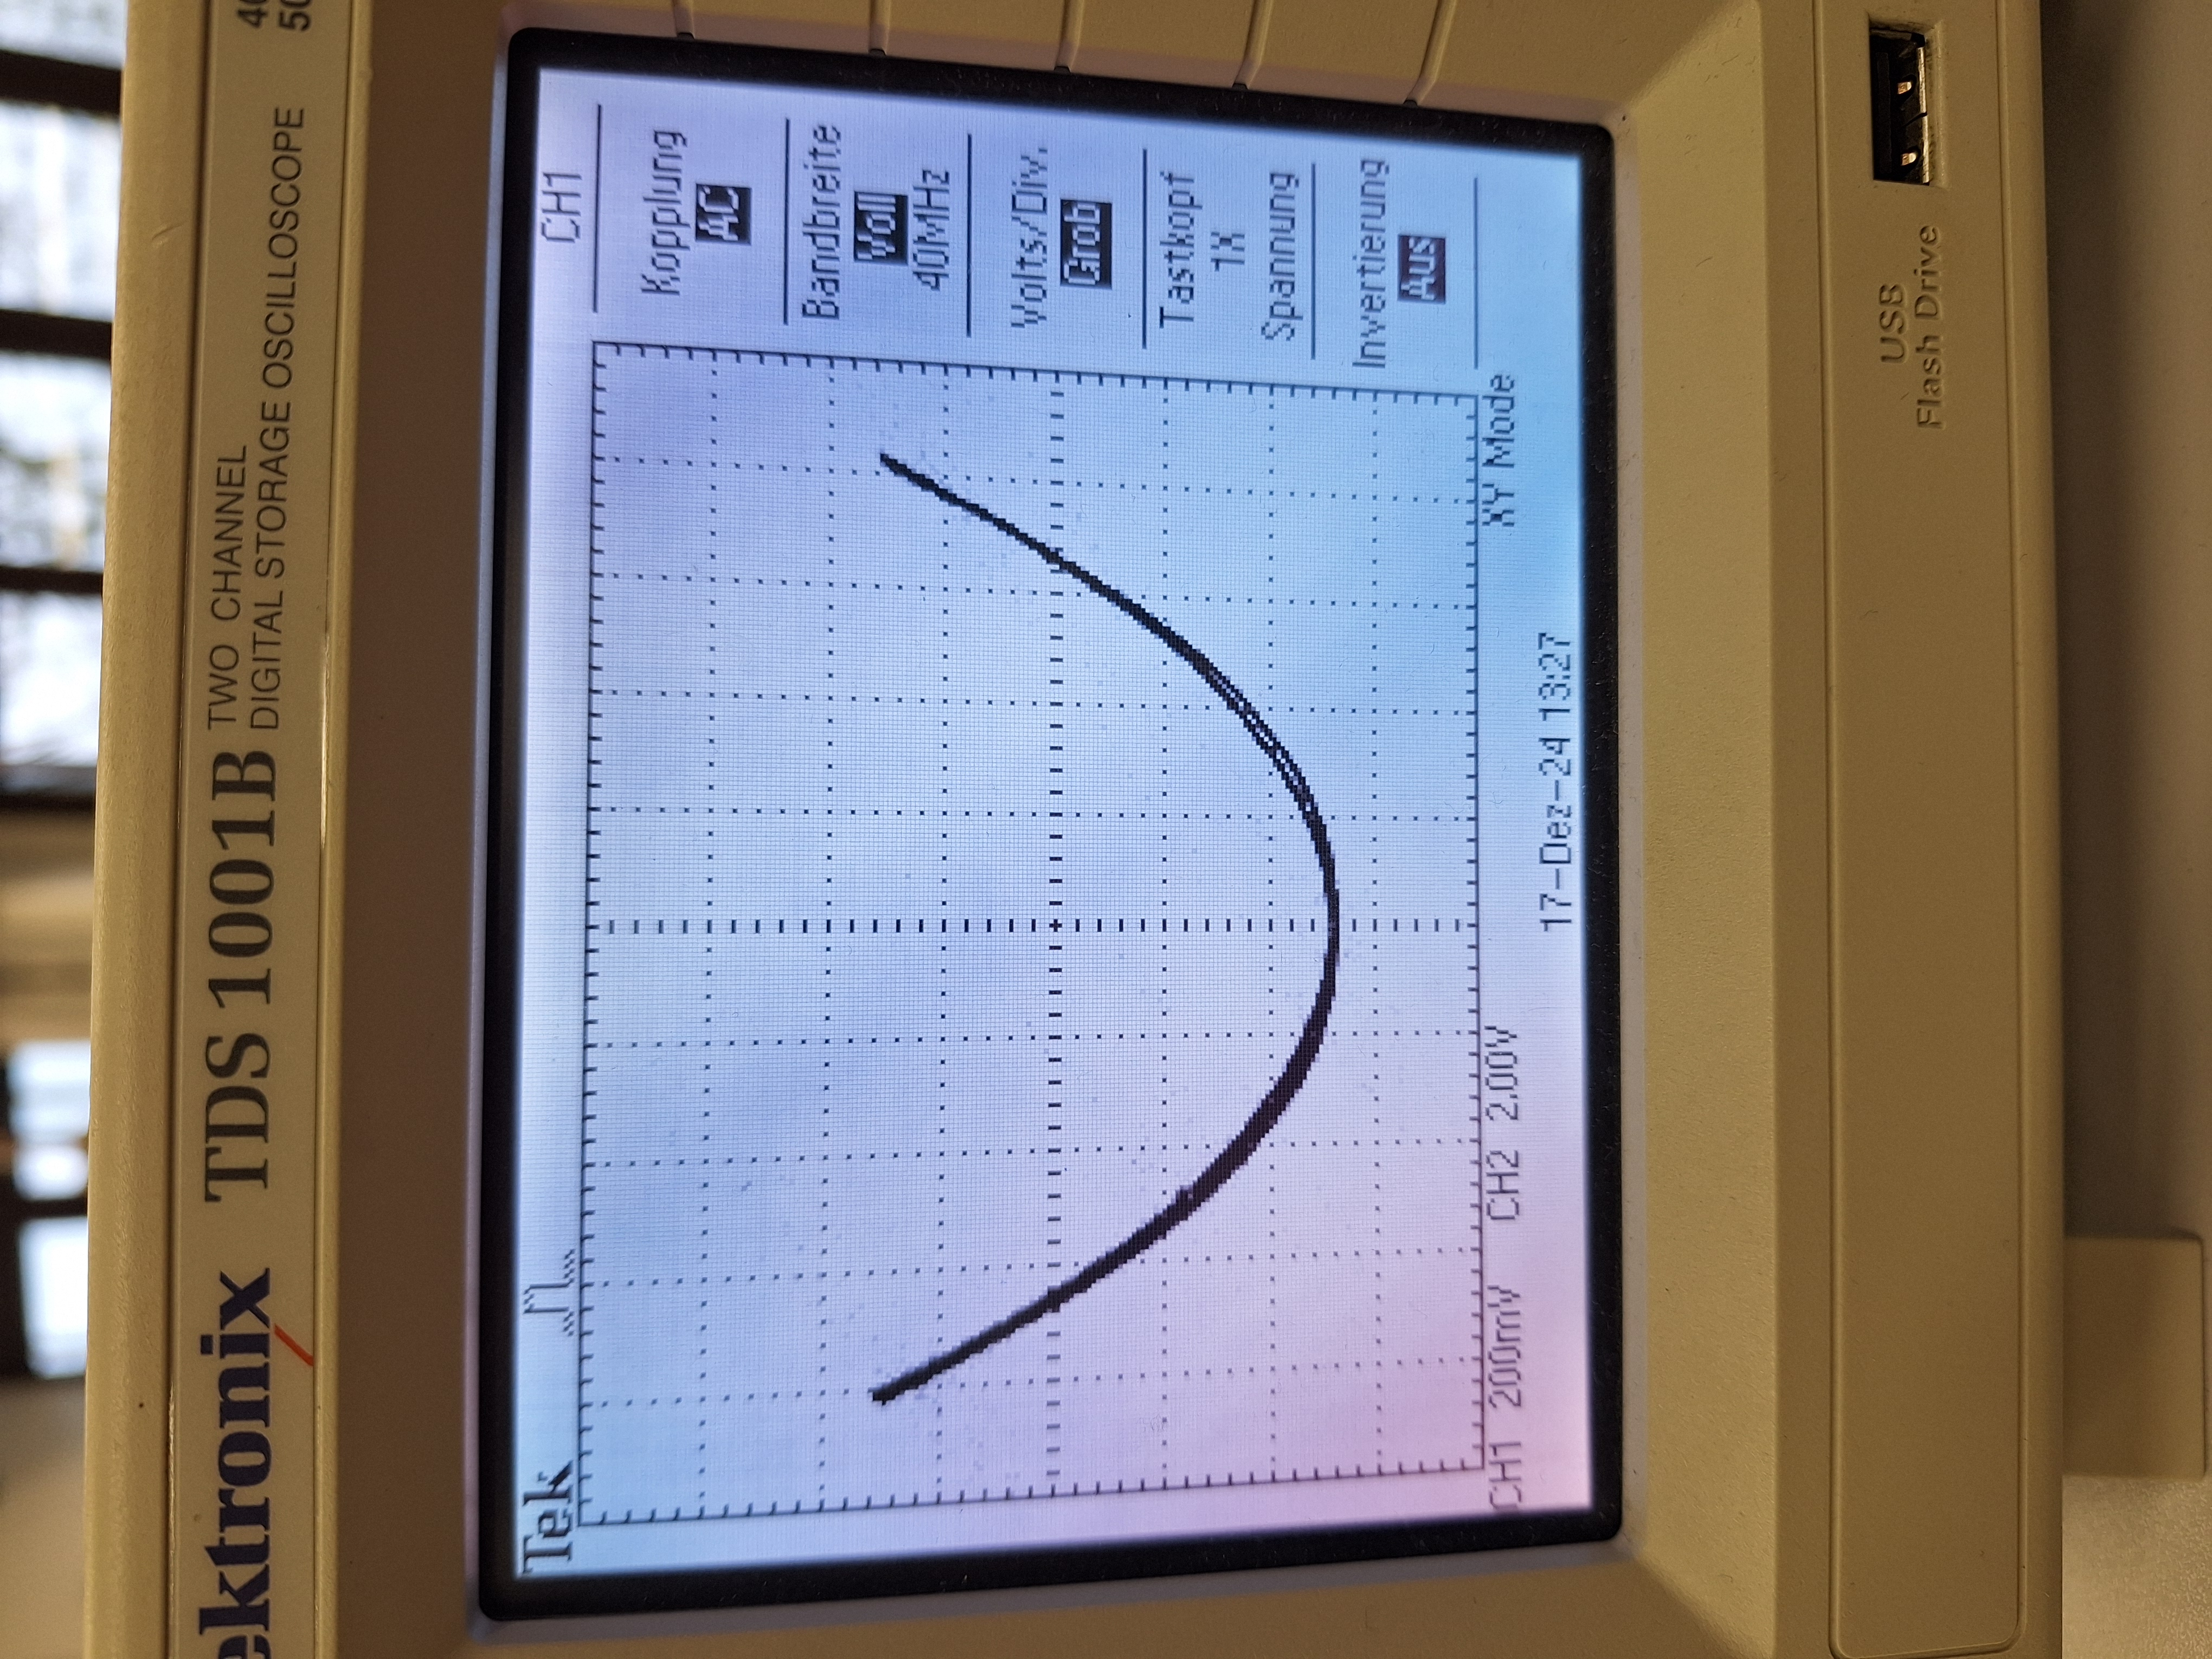
\includegraphics[width=0.9\linewidth, angle=-90]{"Bilder/la.jpg"}
        \caption{Variierte Lissajous-Figur.}
        \label{fig:3}
    \end{minipage}
\end{figure}
\noindent Diese werden abgeglichen, indem das virtuelle Bilder dermaßen geändert wird, 
dass sich die Kurven überlagern wie in \autoref{fig:3} dargestellt.
Für die Sägezahnspannung muss jede Oberwelle ausgegeben gleichzeitig ausgegeben 
und auf dem Oszilloskop angezeigt werden.
Für die Rechteck-und Dreieckspannung reicht es, jede zweite Oberwelle derartig 
zu detektieren.

\subsection{Fourier-Analyse}
Für den zweiten Teil des Experiments werden der Funktionsgenerator und das 
Oszilloskop genutzt. Am Generator wird jeweils eine Dreiecks-, Sägezahn- oder 
Rechteckschwingung eingestellt, am Oszilloskop wird überprüft ob die Schwingung 
übermittelt wird. Im Anschluss wird Fouriertransformation am Oszilloskop
durchgeführt. Am Oszilloskop wird das Frequenzspektrum der Transformation 
abgebildet, welches wie in \autoref{subsec:FTheorem} einer exponentiell abfallenden 
Funktion gleicht. Dabei ist anzumerken, dass die Spektren jeweils ein Rauschen 
beinhalten, welche vernachlässigt werden können. 

\noindent Die Peaks werden in $\unit{\deci\bel}$ aufgenommen und mithilfe des
integrierten Navigators am Oszilloskop abgelesen.